\section{Models}
To represent the real world using equations, we first need to define a model. 
A model is a \textbf{mathematical approximation} of the real world, which allows describing events and phenomena using parametric representations. 
The parameters of the model can be used for processing purposes.

\subsection{Pinhole Camera Model}
The first model we will discuss is the \textbf{pinhole camera model}, which relates to how a camera captures an image. 
It assumes that an object in the real world emits light rays that pass through a small hole (the pinhole) and project onto an image plane, creating an image.

\begin{figure}[H]
    \centering
    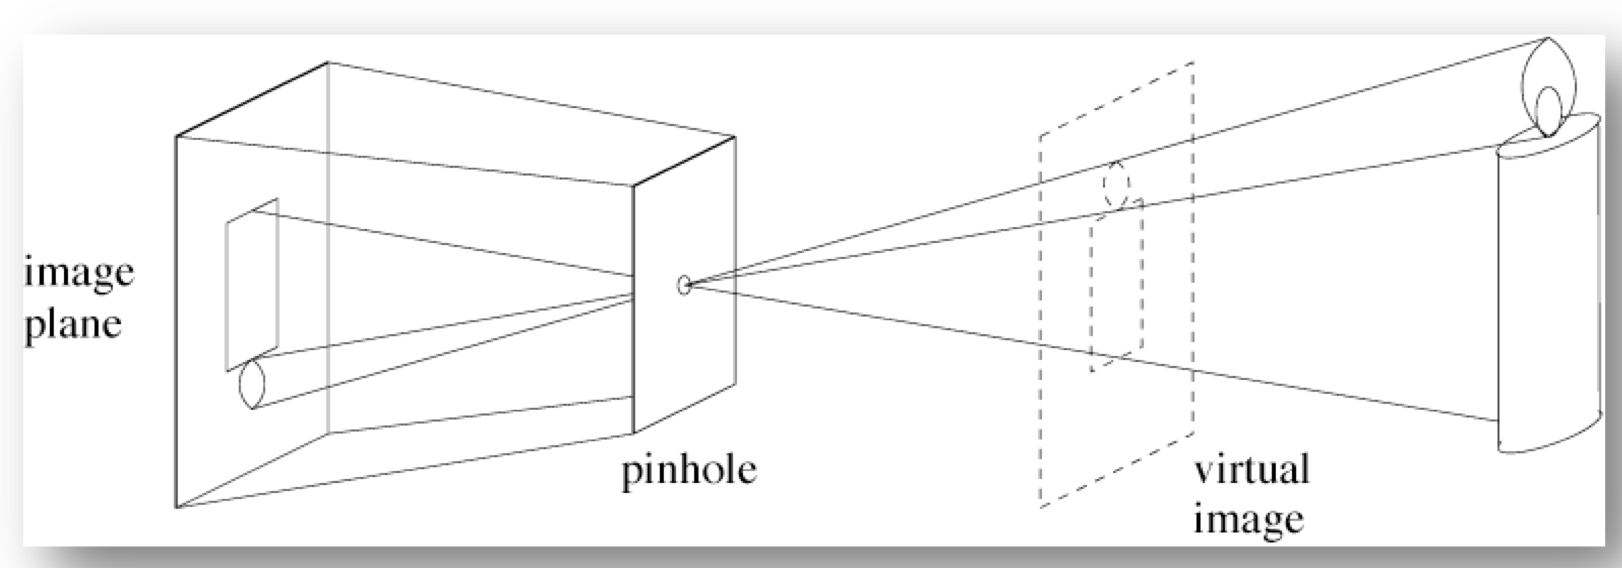
\includegraphics[width=0.5\textwidth]{../media/models/pinhole-camera-model.png}
    \caption{Pinhole Camera Model}
\end{figure}
The pinhole camera model is a simple geometric model that captures the essential features of image formation.

We want to make sure that only a \textbf{single ray of light} from each point of the object passes through the pinhole (ideally, the pinhole should be infinitely small), 
which allows us to create a clear image on the image plane. 
Bigger holes would allow multiple rays from the same point to pass through, resulting in a blurry / out-of-focus image.

On the image plane, the rays of light from the object are projected, creating an image which is flipped upside down. 
Its size is determined by the distance between the object and the pinhole, and the distance between the pinhole and the image plane 
(also known as the \textbf{focal length} $f$). 
The relationship between the object size, the image size, and the distances can be described using similar triangles:

\begin{minipage}{0.45\textwidth}
    \centering
    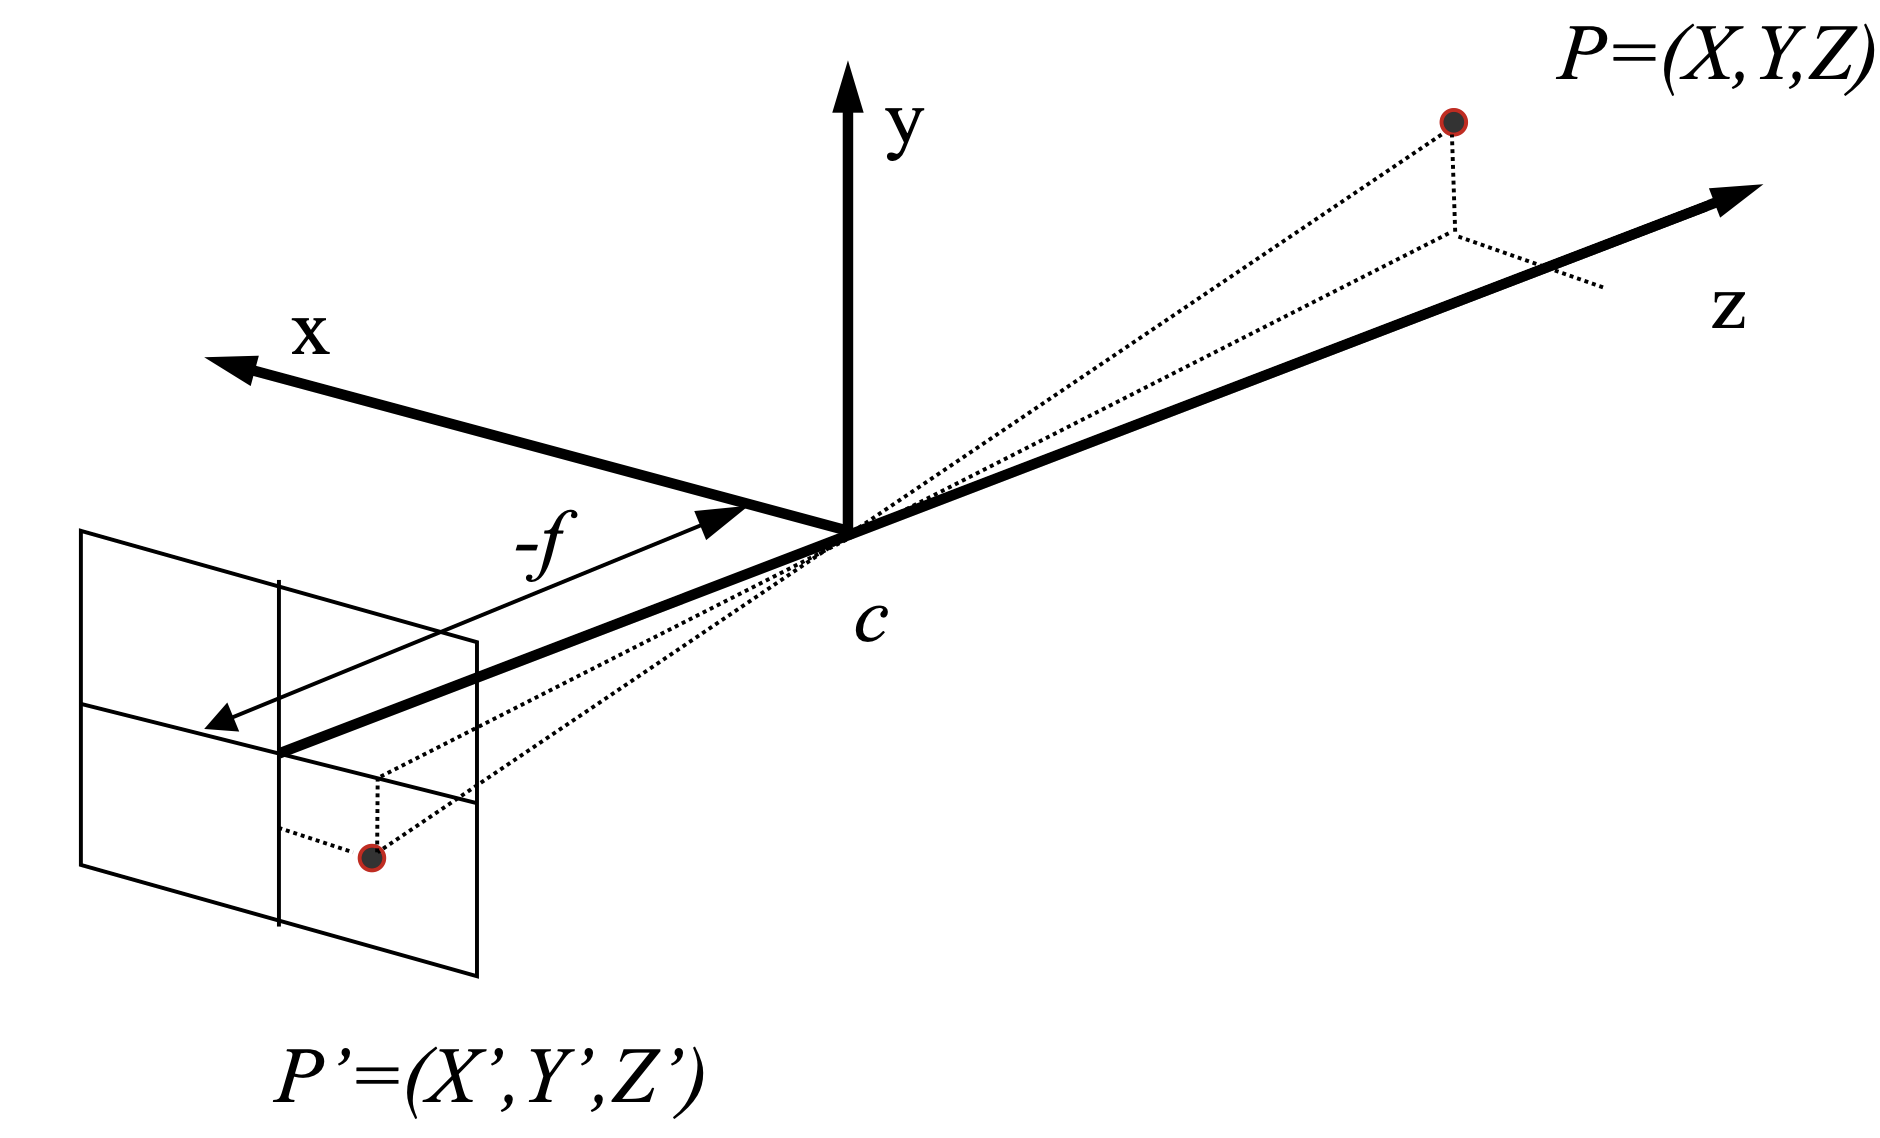
\includegraphics[width=\textwidth]{../media/models/projection.png}
    \captionof{figure}{Projection of the point $P$ onto the image plane}
\end{minipage}
\hfill
\begin{minipage}{0.45\textwidth}
    \centering
    \scalebox{0.8}{
        \begin{tikzpicture}
    %Define the z axis
    \draw[->, thick] (-3,0) -- (3,0) node[right] {$z$};
    %Define the y axis
    \draw[->, thick] (0,-2) -- (0,2) node[above] {$y$};

    % Add the point P
    \filldraw[black] (2.5,1) circle (2pt) node[above right] {$P = (X, Y, Z)$};
    % Add the point projection P'
    \filldraw[black] (-1.5,-0.6) circle (2pt) node[below left] {$P' = (X', Y', Z')$};
    % Add the trajectory of the ray from P to P'
    \draw[dotted, thick] (2.5,1) -- (-1.5,-0.6);

    % Add the pinhole at the origin c
    \filldraw[black] (0,0) circle (2pt) node[below right] {$C$};

    % Add the focal length f
    \draw[dotted, thick] (0,0) -- (-2.5,0) node[midway, above] {$-f$};

    %Add the projections of triangles
    \draw[dotted, thick] (2.5,1) -- (2.5,0);
    \draw[dotted, thick] (2.5,0) -- (0,0);
    \draw[dotted, thick] (-1.5,-0.6) -- (-1.5,0);
    \draw[dotted, thick] (-1.5,0) -- (0,0);
\end{tikzpicture}
    }
    \captionof{figure}{Projection of the point $P$ onto the image plane (2D representation)}
\end{minipage}

\vspace{1em}
As shown in the figure, the point $P$ in the real world is projected onto the image plane as $P'$. The coordinates of $P'$ can be obtained using the geometric properties of the pinhole camera model. The triangles formed by the points $P$, $C$ (the pinhole), and $P'$ are similar, which means that the ratios between the corresponding sides are equal.

This leads to the following relations:
\begin{equation*}
\begin{cases}
Z' = -f \\\\
\dfrac{Z}{Z'} = \dfrac{X}{X'} \\\\
\dfrac{Z}{Z'} = \dfrac{Y}{Y'}
\end{cases}
\end{equation*}

Substituting $Z' = -f$ and rearranging the equations, we obtain:
\begin{align*}
X' &= -f \frac{X}{Z} \\
Y' &= -f \frac{Y}{Z}
\end{align*}

Therefore, the projection of the 3D point $P=(X,Y,Z)$ onto the image plane is given by:
\[
P' = \left(-f \frac{X}{Z},\; -f \frac{Y}{Z},\; -f\right)
\]

\subsubsection{Features of the model}
The pinhole camera model has several important features:
\begin{itemize}
    \item Further objects appear smaller in the image, which is a consequence of the projection process. It is not able to correctly capture depth information directly.
    \item Parallel lines in the real world appear to converge towards a single point in the image, known as the \textbf{vanishing point}. The line connecting the vanishing points is called the \textbf{horizon line}. Vertical lines in the real world will still appear vertical in the image, being perpendicular to the horizon line.
    \item The image is inverted (upside down) due to the way light rays pass through the pinhole.
    \item The model assumes that the pinhole is infinitely small, which is an idealization. This would require an infinite amount of light to pass through to create a visible image, which is not practical.
\end{itemize}

% ---------------------------------------------------------
% LENSES MOVED HERE: Logical progression from Pinhole limitations
% ---------------------------------------------------------
\subsection{Lenses}
Up until now, we have assumed that our cameras were pinhole cameras, which is not the case in the real world. In reality, cameras use \textbf{lenses} to focus light onto the image plane. This allows a wider set of light rays from the same point $P$ to merge at point $P'$ on the image plane, creating a brighter image without losing sharpness—provided the distances obey the \textit{thin lens equation}.

\subsubsection{Thin Lens Equation}
\begin{figure}[H]
    \centering
    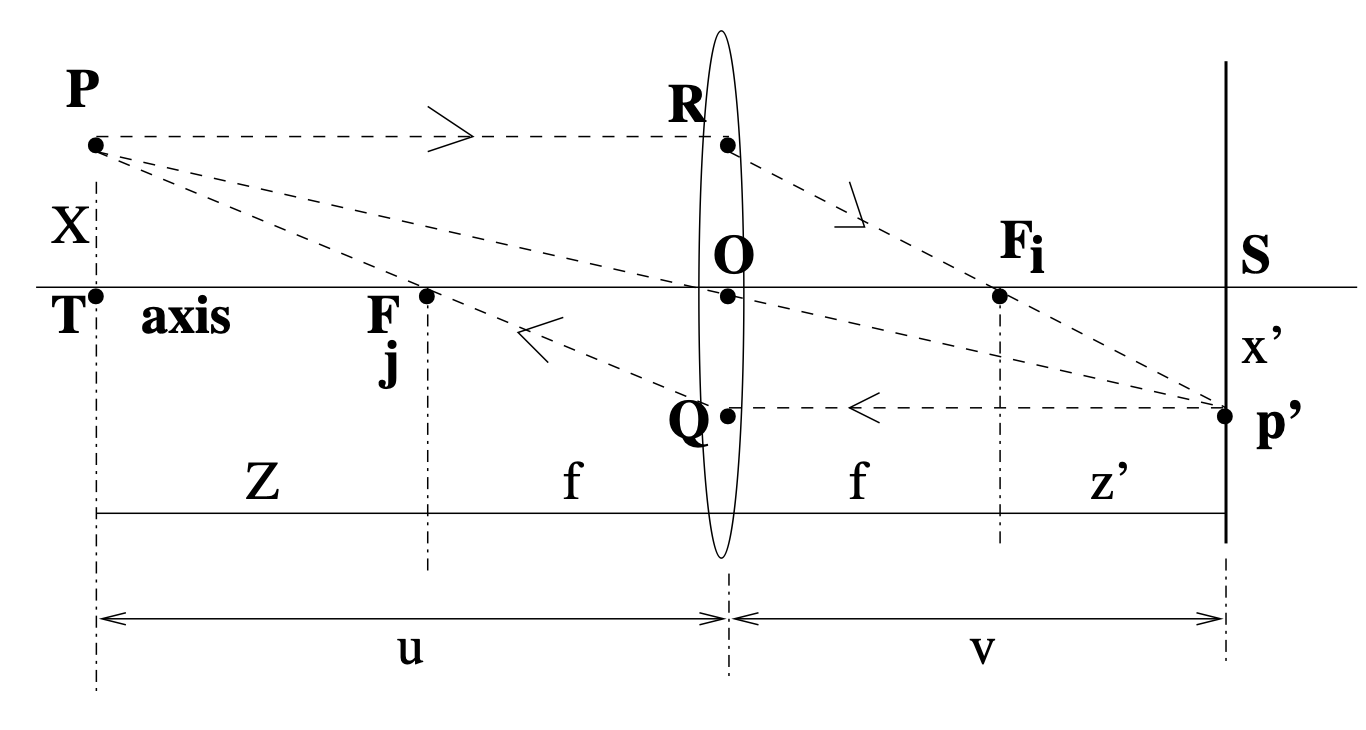
\includegraphics[width=0.5\textwidth]{../media/models/thin_lens.png}
    \caption{Thin Lens model.}
\end{figure}

Suppose we have an object at distance $u$ from the lens, and an image plane at distance $v$ from the lens. Let $X$ be the object height and $X'$ be the projected image height. By considering the similar triangles formed by rays passing through the optical center, we have:
\begin{equation}
    \frac{X}{u} = \frac{X'}{v}
\end{equation}
Considering a second ray passing through the focal point $F$ (at distance $f$ from the lens):
\begin{equation}
    \frac{X}{u - f} = \frac{X'}{f}
\end{equation}
Equating the ratios for $\frac{X}{X'}$, we get:
\begin{equation*}
    \frac{u}{v} = \frac{u - f}{f}
\end{equation*}
Cross-multiplying yields $uf = v(u - f) \implies uf = vu - vf$. Dividing all terms by $uvf$, we arrive at the \textit{thin lens equation}:
\begin{equation}
    \label{eq:thin_lens_equation}
    \frac{1}{f} = \frac{1}{u} + \frac{1}{v}
\end{equation}
This equation describes the relationship between the focal length $f$, the object distance $u$, and the image plane distance $v$. If the object goes to infinity ($u \rightarrow \infty$), the image plane must be located exactly at the focal length ($v = f$).

\subsubsection{Focus \& Depth of Field}
If we move the image plane (changing $v$), the point $P'$ will project to a different area, meaning the objects will be out of focus. Similarly, if $P$ moves (changing $u$), the image plane must be adjusted to keep the object in focus.

\begin{figure}[H]
    \centering
    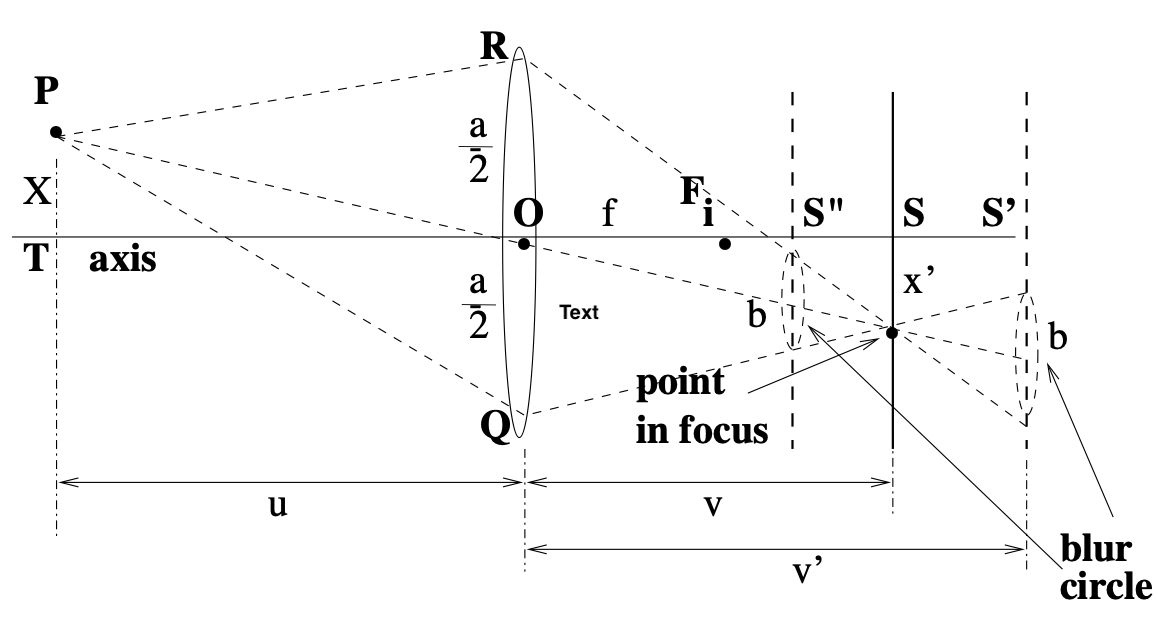
\includegraphics[width=0.5\textwidth]{../media/models/focus.png}
    \caption{Focus and out-of-focus objects.}
\end{figure}

When out of focus, instead of a single point $P'$, we get a \textbf{blur circle} of diameter $b$. We must define an acceptable level of blur. Using the thin lens equation, we can determine the range of distances where objects remain acceptably sharp, known as the \textbf{depth of field}.

Let $a$ be the lens aperture diameter. The range of acceptable image plane distances is:
\begin{equation*}
    \begin{cases}
        v' = \frac{a + b}{a} v  \\\\
        v'' = \frac{a - b}{a} v
    \end{cases}
\end{equation*}
Translating this to object distances gives us the near limit ($u_n$) and far limit ($u_r$) of the depth of field:
\begin{equation*}
    \begin{cases}
        u_n = \frac{u(a+b)}{a+ \frac{bu}{f}} \\\\
        u_r = \frac{u(a-b)}{a- \frac{bu}{f}}
    \end{cases}
\end{equation*}

Notice that:
\begin{itemize}
    \item If $f$ becomes smaller, $u_r$ becomes larger, resulting in a wider depth of field.
    \item If $u \rightarrow \infty$, the rays are parallel, $v = f$, and all distant objects remain in focus.
\end{itemize}

\subsubsection{Autofocus}
Modern cameras use autofocus systems to adjust the image plane position:
\begin{itemize}
    \item \textbf{Active autofocus}: The camera emits a signal (e.g., infrared) and measures the time of flight to estimate distance. It struggles with distant objects, interference, or highly reflective surfaces.
    \item \textbf{Passive autofocus}: The camera analyzes the image itself (often targeting high-contrast edges) to maximize sharpness. 
\end{itemize}

\subsubsection{Resolution, Blur, and Resolving Power}
A camera with an $N \times M$ pixel sensor can detect at most $\frac{N}{2}$ horizontal lines (one pixel must be left between two lines to distinguish them). We define the \textbf{resolving power} $R_p$ as the maximum number of lines per unit distance the camera can distinguish:
\begin{equation}
    R_p = \frac{1}{2\Delta}
\end{equation}
where $\Delta$ is the spacing between two distinguishable lines on the sensor.

\paragraph{Example:}
Consider a $36\text{mm} \times 24\text{mm}$ sensor with a resolution of $4000 \times 2500$ pixels. Calculating vertical $\Delta$:
\begin{equation*}
    \Delta = \frac{24\text{mm}}{2500} \approx 0.01\text{mm}
\end{equation*}
Thus, the resolving power is $R_p = \frac{1}{2 \times 0.01\text{mm}} = 50 \text{ lines/mm}$.

If we capture an object at distance $u = 5000\text{mm}$ with focal length $f = 50\text{mm}$, what is the minimum distinguishable object size?
Rays from adjacent distinguishable lines have an angular separation $\theta$. For small angles:
\begin{equation*}
    2 \Delta \approx f \theta \implies \theta = \frac{2 \Delta}{f} = \frac{0.02\text{mm}}{50\text{mm}} = 0.0004 \text{ radians}
\end{equation*}
The minimum object size is:
\begin{equation*}
    \text{object size} \approx u \theta = 5000\text{mm} \times 0.0004 = 2\text{mm}
\end{equation*}

\subsubsection{Typical Lens Issues}
\begin{itemize}
    \item \textbf{Barrel distortion}: Caused by wide-angle lenses; straight lines curve outward from the center.
    \item \textbf{Chromatic aberration}: Different wavelengths are refracted differently, resulting in color fringing around edges.
    \item \textbf{Vignetting}: Light falloff causes the image corners to appear darker than the center.
\end{itemize}

\subsection{Projection}
By the time we capture an image, we have already projected the 3D world onto a 2D plane. 
Considering the time dimension, we formalize projection as:
\[f: \mathbb{R}^4 \rightarrow \mathbb{R}^3\]
\[ (X, Y, Z, t) \mapsto (x, y, t)\]
We will discuss the two main projection models used in computer vision: \textbf{perspective projection} and \textbf{orthographic projection}.

\subsubsection{Perspective Projection}
Perspective projection models how objects appear smaller as distance increases. 
In this specific coordinate convention, the image plane is at the origin $(0,0,0)$ and the lens center is at $Z = f$.
\begin{figure}[H]
    \centering
    \scalebox{0.8}{
        \input{Tikz/models/perspective-projection-2d.tex}
    }
    \caption{Perspective Projection}
\end{figure}

The similar triangles formed by points $P$, $C$, and $P'$ give:
\begin{equation*}
\begin{cases}
Z' = 0 \\\\
\dfrac{f}{Z - f} = \dfrac{x}{X} \\\\
\dfrac{f}{Z - f} = \dfrac{y}{Y}
\end{cases}
\end{equation*}

Therefore, the projection of $P=(X,Y,Z)$ is:
\[
P' = \left(f \frac{X}{Z - f},\; f \frac{Y}{Z - f},\; 0\right)
\]
Because perspective projection maps infinitely many 3D points lying on the same viewing ray to the same image point, 
depth cannot be recovered from a single image alone without additional constraints or multiple views (e.g., stereo vision).

\subsubsection*{Simplified Perspective Projection}
To avoid an inverted image, we can place a virtual image plane in front of the lens at distance $f$.
\begin{figure}[H]
    \centering
    \scalebox{0.8}{
        \begin{tikzpicture}
    %Define the z axis
    \draw[->, thick] (-3,0) -- (3,0) node[right] {$z$};
    %Define the y axis
    \draw[->, thick] (0,-2) -- (0,2) node[above] {$y$};

    % Add the point P
    \filldraw[black] (2.5,1) circle (2pt) node[above right] {$P = (X, Y, Z)$};
    % Add the point projection P'
    \filldraw[black] (1.5,0.6) circle (2pt) node[above left] {$P' = (x, y, z)$};
    % Add the trajectory of the ray from P to C
    \draw[dotted, thick] (2.5,1) -- (0,0);

    % Add the pinhole at the origin c
    \filldraw[black] (0,0) circle (2pt) node[below right] {$C$};

    % Add the focal length f
    \filldraw[black] (1.5,0) circle (2pt) node[below] {$f$};

    %Add the projections of triangles
    \draw[dotted, thick] (2.5,1) -- (2.5,0);
    \draw[dotted, thick] (2.5,0) -- (0,0);
    \draw[dotted, thick] (1.5,0.6) -- (1.5,0);
\end{tikzpicture}
    }
    \caption{Simplified Perspective Projection.}
\end{figure}

The simplified equations map the 3D point $P=(X,Y,Z)$ to:
\[P' = \left(f \frac{X}{Z},\; f \frac{Y}{Z},\; 0\right)\]
This simplification is highly practical and standard when $f \ll Z$.

\subsubsection{Orthographic Projection}
Orthographic projection assumes that light rays generated by the scene are parallel and perpendicular to the image plane. 
This allows for a simple projection where perspective distortion is ignored.
\begin{figure}[H]
    \centering
    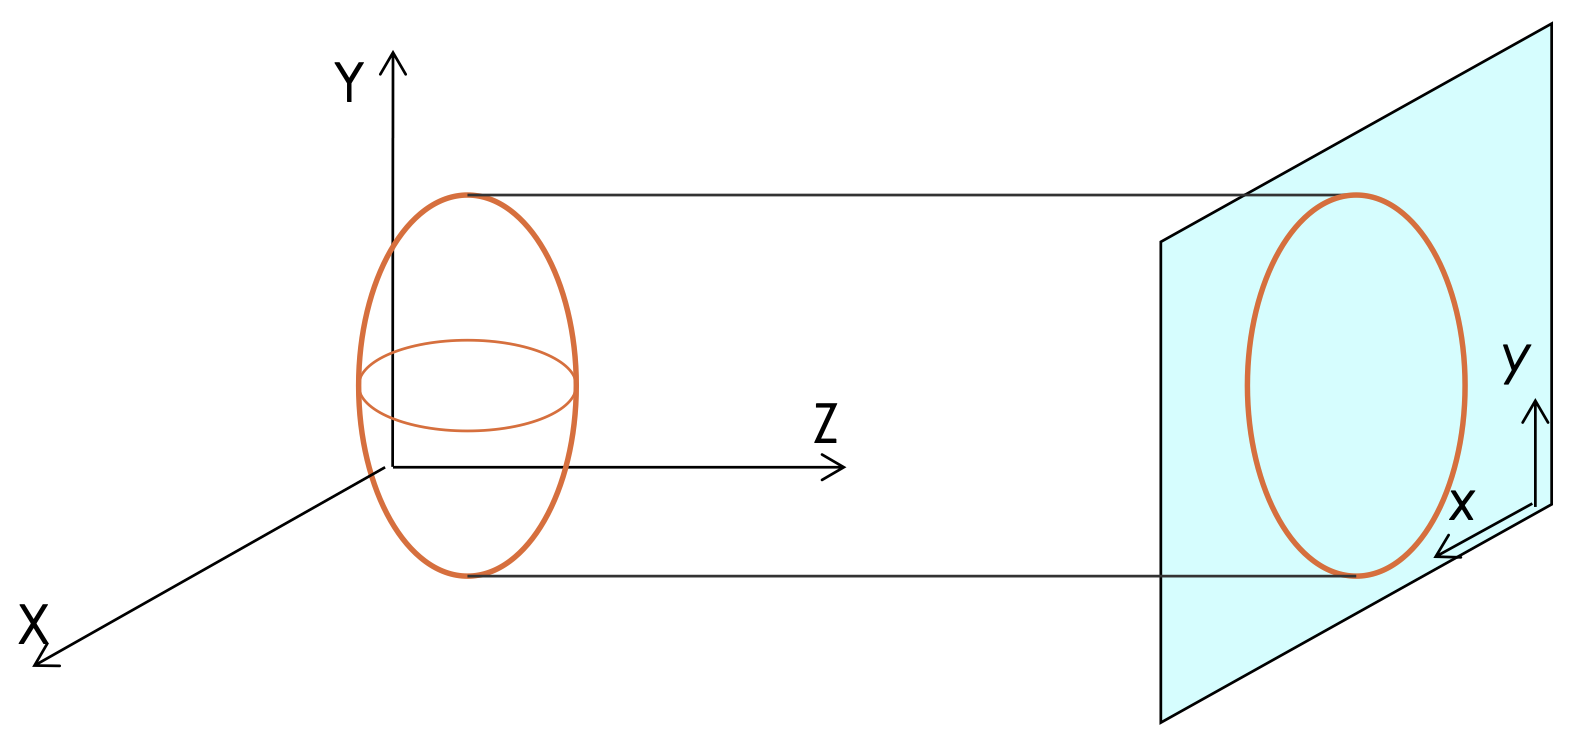
\includegraphics[width=0.5\textwidth]{../media/models/orthographic-projection.png}
    \caption{Orthographic Projection model.}
\end{figure}

This is valid when the object's depth is negligible compared to its distance from the camera (e.g., satellite imaging).
\[P' = (X, Y, 0)\]
In matrix form:
\[
    \begin{bmatrix} x \\ y \end{bmatrix} = \begin{bmatrix} 1 & 0 & 0 \\ 0 & 1 & 0 \end{bmatrix} \begin{bmatrix} X \\ Y \\ Z \end{bmatrix}
\]

\subsection{Illumination Model}
Once geometry is established, illumination dictates the pixel intensities. Light hitting an object can be \textbf{absorbed}, \textbf{reflected}, or \textbf{transmitted}. Cameras rely purely on reflected light.

\subsubsection{Reflection Types}
\begin{itemize}
    \item \textbf{Specular}: Energy is concentrated in a specific direction (glossy surfaces).
    \item \textbf{Diffuse}: Energy is scattered uniformly in all directions (matte surfaces). Observer position is irrelevant.
\end{itemize}

\subsubsection{Lambertian Reflectance Model}
Assuming a distant, single light source, rays are parallel. For a perfectly diffuse (Lambertian) surface, the reflected intensity $i$ is proportional to the cosine of the angle $\alpha$ between the \textbf{surface normal} $n$ and the \textbf{light direction} $s$ (Lambert's Cosine Law).

The model is expressed as:
\begin{equation}
    \label{eq:lambertian_reflectance_model}
    i = \rho (s \cdot n)
\end{equation}
which expands to:
\[ i = \rho \|n\| \|s\| \cos(\alpha)\]
where $\rho$ is the surface \textit{albedo} (the fraction of reflected light). 

If $s \cdot n \le 0$, the normal points away from the light source, meaning the point is in shadow and not illuminated.